The proposed rover redesigns and \ac{SA} configurations for both mission sites are modeled with Blender/Phobos. Phobos is ``an add-on for the open-source 3D modeling software Blender that enables the creation of robot models for use in robot frameworks like ROS and ROCK or in real-time simulations such as MARS'' \citeother{Phobos}. MARS is ``a cross-platform simulation and visualisation tool created for robotics research. It consists of a core framework containing all main simulation components, a GUI (based on Qt), 3D visualization (using OSG) and a physics engine (based on ODE)'' \citeother{MARSSim}. \refFig{fig:simulated-mission-site-ismenius-cavus} shows the robot model loaded on the MARS platform to simulatie mission scenarios using a \ac{HiRISE} \ac{DTM} of a well preserved crater at Ismenius Cavus.  The simulated solar power output data is produced by a \ac{PMS} implemented as part of this thesis which is integrated with the already available robot simulation toolkit.

\begin{figure}[h]
  \captionsetup[subfigure]{justification=centering}
  \centering
  \hypersetup{linkcolor=captionTextColor}
  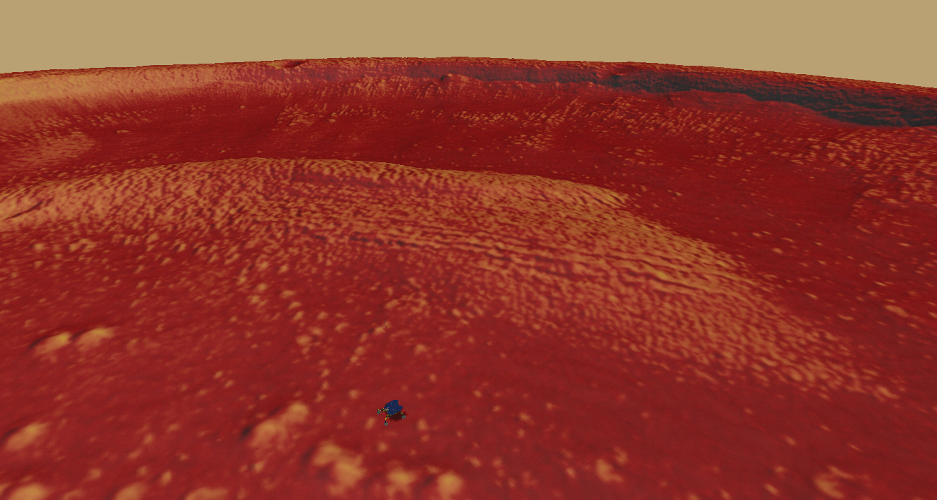
\includegraphics[width=1\linewidth]{sections/design/simulation/images/mars-sim-ismenius-cavus.png}\\
  \caption[Simulation of the rover inside a well preserved crater at Ismenius Cavus]
          {Simulation of the rover inside a well preserved crater at Ismenius Cavus.}
  \label{fig:simulated-mission-site-ismenius-cavus}
\end{figure}

\subsection{Z-Axis Revolutions}

\refFig{fig:simulation-data-rover-revolution-generated-power} and \refFig{fig:simulation-data-rover-revolution-generated-power-polar} are two different representations of the same solar generated power data obtained from commanding the rover to execute a \SI{10}{\degree} forward body-pitch followed by several revolutions around its z-axis. These revolutions result in a sinusoidal generated power variation.

\begin{figure}[h]
  \captionsetup[subfigure]{justification=centering}
  \centering
  \hypersetup{linkcolor=captionTextColor}
  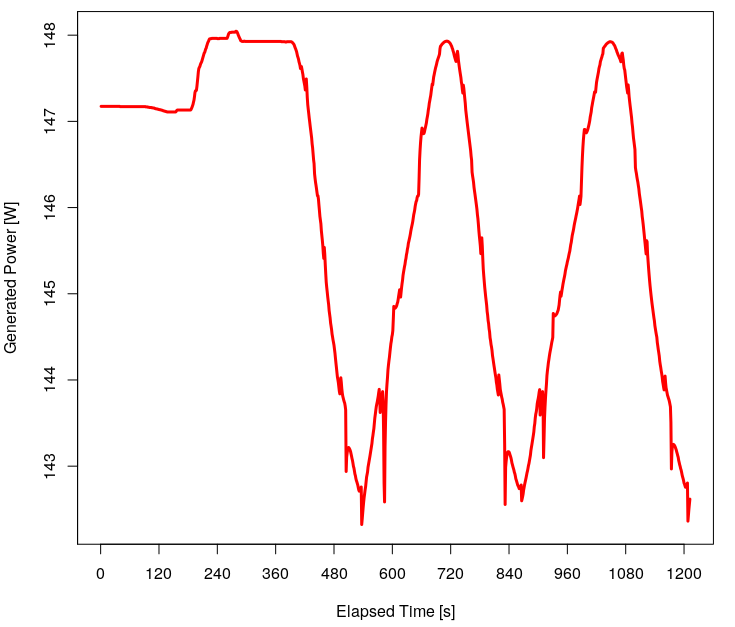
\includegraphics[width=0.5\linewidth]{sections/design/simulation/plots/rover-generated-power.png}\\
  \caption[Power generated by the rover's solar array for multiple revolutions along its z-axis]
          {Power generated by the rover's solar array for multiple revolutions along its z-axis. Simulation conditions is solar noon at Ismenius Cavus.}
  \label{fig:simulation-data-rover-revolution-generated-power}
\end{figure}

In \refFig{fig:simulation-data-rover-revolution-generated-power-polar}, the angle values represent the direction faced by the inclined solar array. Maximum power is generated when the rover's solar panels are facing South towards the equator. Inversely, facing northwards away from the equator genrates the least amount of power.


\begin{figure}[h]
  \captionsetup[subfigure]{justification=centering}
  \centering
  \hypersetup{linkcolor=captionTextColor}
  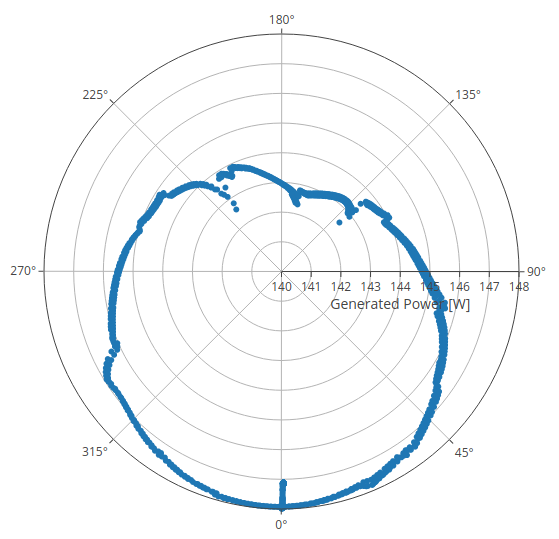
\includegraphics[width=0.4\linewidth]{sections/design/simulation/plots/rover-revolution-generated-power.png}\\
  \caption[Polar visualization of power generated by the rover's solar array for multiple revolutions along its z-axis]
          {Polar visualization of power generated by the rover's solar array for multiple revolutions along its z-axis. Angle values represent the direction faced by the inclined solar array. \SI{0}{\degree} is South, \SI{90}{\degree} is East, \SI{180}{\degree} is North, and \SI{270}{\degree} is West. Simulation conditions is solar noon at Ismenius Cavus.}
  \label{fig:simulation-data-rover-revolution-generated-power-polar}
\end{figure}

\clearpage
\subsection{Slope Compensation}

\refFig{fig:rover-counter-slope} shows a simulated scenario in which the rover is on a \SI{30}{\degree} inclined slope. The slope's inclination is facing opposite the equator resulting in a worst case power generation. The rover is positioned with a backward body-pitch of \SI{10}{\degree} in order to counter the slope induced forward inclination thus reducing \ac{SA} inclination angle from $\beta=\SI{30}{\degree}$ to $\beta=\SI{20}{\degree}$.

\begin{figure}[h]
  \captionsetup[subfigure]{justification=centering}
  \centering
  \hypersetup{linkcolor=captionTextColor}
  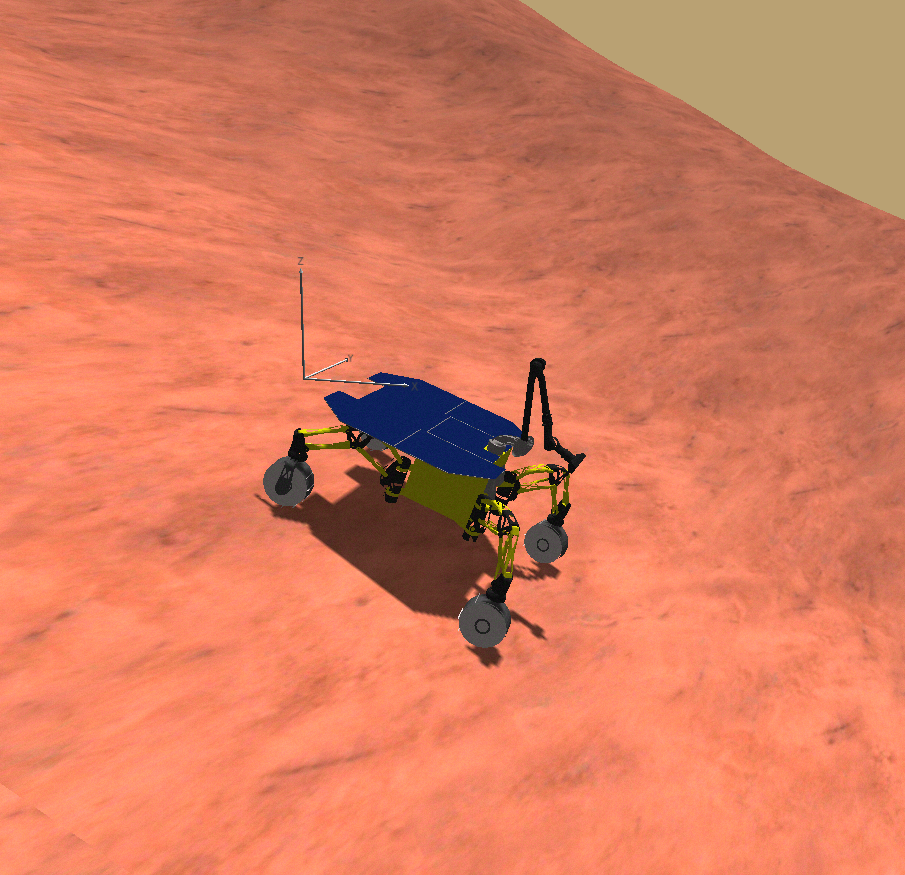
\includegraphics[width=0.4\linewidth]{sections/design/simulation/images/counter-slope.png}\\
  \caption[Simulation of the rover on an inclined slope.]
          {Simulation of the rover on an inclined slope.}
  \label{fig:rover-counter-slope}
\end{figure}

\refFig{fig:rover-counter-slope-measurements} shows solar power outputs for different body-pitch configuration while the rover is on a \SI{30}{\degree} slope. The initial state of the body-pitch is \SI{0}{\degree} follow by two seperate \SI{5}{\degree} forward pitch increments which worsen solar power generation by changing $\beta=\SI{30}{\degree}$ to $\beta=\SI{40}{\degree}$. After which, four separate \SI{5}{\degree} backward pitch decrements are executed, progressively improving power generation as $\beta$ is changed from \SI{40}{\degree} to \SI{20}{\degree}. As a final task, the rover is commanded to drive forward and it encounters uneven terrain which introduces minor fluctuations to the solar power output.

\vspace{0.5cm}

\begin{figure}[h]
  \captionsetup[subfigure]{justification=centering}
  \centering
  \hypersetup{linkcolor=captionTextColor}
  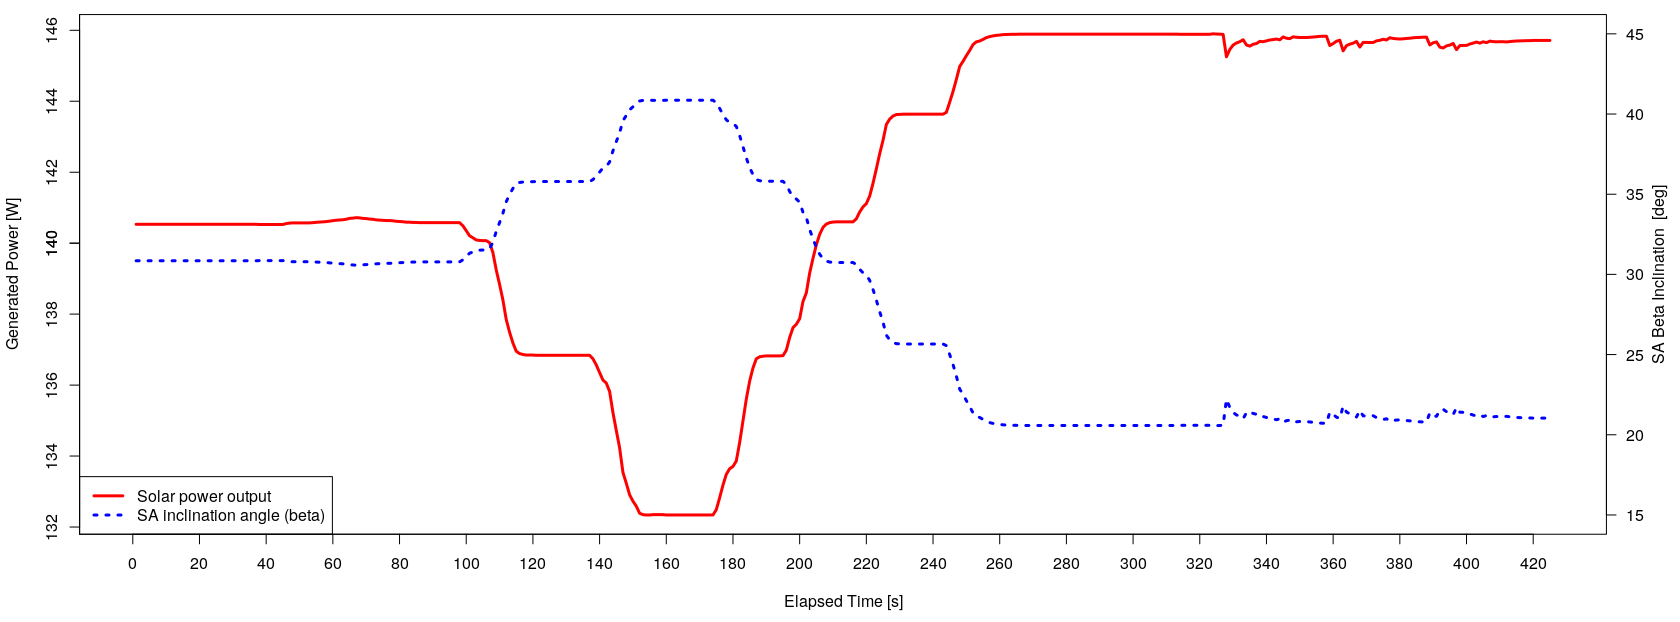
\includegraphics[width=0.9\linewidth]{sections/design/simulation/plots/counter-slope-plot.png}\\
  \caption[Solar power generated on sloped terrain with different SA inclinations.]
          {Solar power generated on sloped terrain with different SA inclinations.}
  \label{fig:rover-counter-slope-measurements}
\end{figure}
